\documentclass{sig-alternate}

\usepackage[usenames, dvipsnames]{color}
%\usepackage{times}
\usepackage{xspace}
\usepackage{textcomp}
\usepackage{wrapfig}
\usepackage{url}
\usepackage{amsmath, amssymb}
%\usepackage[protrusion=true,expansion=true]{microtype}
%\usepackage{float}
\usepackage{alltt}
\usepackage{appendix}
%\usepackage{algorithm}
\usepackage{algorithmicx}
\usepackage{algpseudocode}
%\usepackage{texlive-science}
\usepackage{comment}

\pdfinfo{/Title (A Deterministic PTIME Language for Asynchronous Distributed Systems)}

\usepackage{txfonts}
\newcommand{\Tau}{\mathcal{T}}
\newcommand{\SDedalus}{\mathcal{S}}
\newcommand{\Consts}{\mathcal{C}}
\newcommand{\Vars}{\mathcal{A}}
%\newcommand{\pos}{\protect{$_{pos}$}}
%\newcommand{\nega}{\protect{$_{neg}$}}
% RCS: Would like to use the above ones, but can't get them to work in Dedalus env.
\newcommand{\pos}{\_pos}
\newcommand{\nega}{\_neg}
\newcommand{\eat}[1]{}

\newcommand{\jmh}[1]{{\textcolor{ForestGreen}{#1 -- jmh}}}
\newcommand{\paa}[1]{{\textcolor{blue}{#1 -- paa}}}
\newcommand{\nrc}[1]{{\textcolor{magenta}{#1 -- nrc}}}
\newcommand{\wrm}[1]{{\color{BurntOrange}{#1 -- wrm}}}
\newcommand{\todo}[1]{{\color{Red}{\textbf{TODO: #1}}}}
\newcommand{\smallurl}[1]{{\small \url{#1}}}

\newtheorem{theorem}{Theorem}
\newtheorem{lemma}{Lemma}
\newtheorem{corollary}{Corollary}
%\theoremstyle{definition}
\newdef{example}{Example}
\newdef{definition}{Definition}

\def\slang{\textsc{Dedalus}$^C$\xspace}
\def\lang{\textsc{Dedalus}\xspace}
%\def\slang{\textsc{Dedalus\ensuremath{_{{0}}}}\xspace}
%\def\synclang{{Dedalus\ensuremath{_{\large 0}}}\xspace}
\newcommand{\naive}      {na\"{\i}ve\xspace}
\newcommand{\Naive}      {Na\"{\i}ve\xspace}
%dedalus environment for code

\newenvironment{Dedalus}{
\vspace{0.5em}\begin{minipage}{0.95\textwidth}%\linespread{1.3}
\begin{alltt}\fontsize{9pt}{9pt}\selectfont}
{\end{alltt}\end{minipage}\vspace{0.5em}}

\newcommand{\dedalus}[1]{\texttt{\fontsize{9pt}{9pt}\selectfont #1}}
\newcommand{\dbar}[1]{\(\bar{\text{\dedalus{#1}}}\)}

\begin{document}

%\conferenceinfo{ACM PODS}{'10 Indianapolis, IN, USA}
\title{A Deterministic PTIME Language for Asynchronous Distributed Systems}
%%Format\titlenote{(Produces the permission block, copyright information and page numbering). For use with ACM\_PROC\_ARTICLE-SP.CLS V2.6SP. Supported by ACM.}}
%
% You need the command \numberofauthors to handle the "boxing"
% and alignment of the authors under the title, and to add
% a section for authors number 4 through n.

\numberofauthors{6}

\author{
%
William R. Marczak \quad Peter Alvaro \quad Joseph M. Hellerstein \quad Neil Conway
\\\\
%
\fontsize{10}{10}\selectfont\itshape 
%\vspace{0.05in}
University of California, Berkeley\\\\ \fontsize{9}{9}\selectfont\ttfamily\upshape
%
\{wrm,palvaro,hellerstein,nrc\}@cs.berkeley.edu
%
}

\toappear{}

\maketitle

\begin{abstract} 
  Building on recent interest in distributed logic programming, we take a
  model-theoretic approach to the correctness of asynchronous distributed
  programs.  We show that the features added in Dedalus, a language previously
  proposed as an extension of Datalog for modeling asynchronous distributed
  programs, increase the expressivity beyond PTIME and allow the specification
  of programs that have non-deterministic results.  As non-determinism is
  undecidable \nrc{This is strangely worded. What do you mean, exactly?}, we
  present a restriction of Dedalus -- which restricts Dedalus to be inflationary
  and removes negation -- that is both deterministic and PTIME.  We add back a
  stratified negation semantics based on practice in the distributed systems
  community.

%
%We present a formal definition of the \lang language and prove conjectures.

% An increasing amount of interest surrounds the use of logic languages such as
% Datalog to ease the design and verification of asynchronous distributed
% systems.  An oft-cited reason is the model-theoretic semantics of logic
% programming, which underpin a robust literature on analysis techniques to
% ensure, among other things, termination and the existince and uniqueness of a
% program result.  While prior work on logic programming for distributed systems
% has demonstrated compactness of representation and efficiency of execution, the
% tantalizing possibility of leveraging model theory to realize analysis
% techniques for distributed systems correctness criteria has gone largely
% unrealized.  In this paper, we define model-theoretic notions for two such
% criteria popular in the distributed systems domain: {\em determinism} and {\em
% eventual consistency}.  Unfortunately, we show that these are undecidable
% properties in the general case.  However, we prove the conjectured result that
% {\em monotonicity} of logic can be a powerful conservative test for these
% criteria, and we leverage existing static {\em stratification} checks from
% logic programming to enforce monotonicity in a large class of programs by
% instrumenting them with {\em coordination logic}.

%However, using analyses from logic programming, including {\em stratification} analyses, 

%Recent distributed systems research has used variants of Datalog to specify and implement large-scale practical systems, showing orders of magnitude reduction in code size~\cite{boon}, and in some cases applying or reinterpreting 

%Programs written in declarative logic languages such as Datalog have a model-theoretic semantics that
%is independent of how the program is executed.  As a result, they are amenable to simple and powerful
%static analysis techniques to ensure, among other things, termination and the existence and uniqueness
%of a program result.  Recent distributed systems research has experimented with using variants of 
%Datalog to specify and implement large-scale practical systems, in some cases applying or reinterpreting
%existing analyses with respect to the new domain~\cite{dedalus}.  

%Continuing in this vein, it is only natural 
%to ask to what extent we can characterize notions of correctness and ``good behavior'' that are unique to distributed 
%systems, like determinism of distributed computations and eventual consistency of replicated state,
% in a model theoretic framework, and whether we may add or adapt program analyses for these properties.

%In this paper, we define a model-theoretic notions of {\em confluence, consistency} and {\em eventual
%consistency}, which are based on the existence of an {\em ultimate models}, or equivalence classes among 
%distributed traces \paa{ummmm}.  We show that for programs that do not have a unique ultimate model, 
%there often exists a single ultimate model that corresponds to the intuitive semantics of the program,
%and which can be enforced via a program rewrite that adds additional {\em coordination} logic to the given
%program to suppress the other models.  We also show that in general, the problem of deciding whether a program
%is consistent or confluent for all EDBs is undecidable, and as a correlary that it is impossible in general to
%soundly and completely verify that a program is correctly ``coordinated.''  
%Nevertheless, we propose a set of conservative tests that suffice for a wide variety of practical systems.
%
\end{abstract}

\section{Introduction}
\wrm{goldilocks argument}

There is widespread belief that the foundations of distributed data management
are a poor fit to popular new platforms for distributed
computing~\cite{ladis}. Classical protocols for transactional atomicity and
distributed consensus rely on timely messaging. But typical modern platforms
consist of thousands of machines in datacenters spread across the world and
exhibit relatively frequent message delays and component failures.  As a result,
many programmers today avoid classical protocols and attempt to build
applications that operate correctly using only loose notions of data
consistency.  While there are software engineering patterns to inform this
process~\cite{quicksand}, there is a need for formal tools to help programmers
reason about distributed data management at the application level.

In recent years there has been revived interest in logic programming as a framework for developing distributed systems (e.g.,~\cite{reactors,boom}).  This has led in turn to optimism about using database theory as a foundation for modeling key correctness issues in distributed programs~\cite{declarative-imperative}.
In this paper we report concrete progress on this front.  

Utilizing a model-theoretic framework for analyzing distributed programs, we demonstrate the undecidability of tests for two key properties of distributed programs: confluence in the face of message delays and reordering, and eventual consistency of replicas.  We then use the same framework to derive a number of constructive results that follow from earlier conjectures~\cite{declarative-imperative}.
First, we demonstrate that distributed programs satisfying a broad definition of  monotonicity are guaranteed to be confluent, producing consistent results in the face of arbitrary message delays and reordering.  We then turn our attention to non-monotonic programs, and provide a generic construction for distributed coordination that guarantees adherence to a natural semantic interpretation.  Finally, we show how to guarantee the eventual consistency of distributed replicas by rewriting programs with a simple generic protocol for data replication.

To connect these results to traditional imperative models of distributed programming, we provide a mapping from our logical framework to a more traditional state-machine model.  In concurrent work we have also used these results directly, to develop practical software analysis tools for distributed logic programming~\cite{cidr11}.  

\subsection{Organization}
In Section~\ref{sec:foundation} we introduce \lang, the distributed logic programming language that we use throughout the paper.  Section~\ref{sec:operational} presents an operational interpretation of a distributed system, and proves a correspondence between \lang models and operational behavior.  We present our confluence results in section~\ref{sec:confluence}, and in Section~\ref{sec:consistency} we examine the issue of replica consistency.  We conclude with a discussion of related and future work (Sections~\ref{sec:relwork} and~\ref{sec:conclusion}).

\section{\large \bf \lang}
\label{sec:foundation}

\subsection{Preliminary Definitions}

We assume an infinite universe $\mathcal{U}$.

A {\em relation schema} is a pair consisting of a relation name and its arity.  A {\em schema} $\mathcal{S}$ is a set of relation schemas.  As in \wrm{cite Immerman}, we assume the existence of an order.  Thus, all schemas contain the following relational schemas: \dedalus{lt} -- a relation of arity two that is true whenever the second argument is greater than the first (we will write this relation in infix form using the \dedalus{<} symbol) -- \dedalus{suc} -- a relation of arity two that defines a total order over $\mathcal{U}$ \wrm{different from succ}.

A {\em rule} over a schema $\mathcal{S}$ is a clause of the form:

\begin{Dedalus}
p(\(\bar{X_0}\)) <- b_1(\(\bar{X_1}\)), \ldots, b_n(\(\bar{X_n}\)), !c_1(\(\bar{Y_1}\)), \ldots, !c_m(\(\bar{Y_m}\)).
\end{Dedalus}

where \dedalus{h}, \dedalus{\(b_1\), \ldots, \(b_n\)}, \dedalus{\(c_1\), \ldots, \(c_m\)} are relations in $\mathcal{S}$, and $\bar{X_i}$ and $\bar{Y_i}$ denote a tuple (of the appropriate arity) consisting of variable symbols, constants from $\mathcal{U}$.  Note that we maintain the usual safety restrictions of Datalog rules: any variable symbol $V$ that appears in $\bar{Y_i}$ for some $1 \leq i \leq m$ must also appear in $\bar{X_j}$ for some $1 \leq j \leq n$, but only if $V$ appears in $\bar{X_0}$ or $V$ appears in $\bar{Y_k}$ for some $k \neq i$ -- i.e., variable symbols that only appear in a single negated atom and do not appear in the head need not also appear in a positive atom \wrm{cite ullman}.

\wrm{describe recursion, rule out recursion through negation, define EDB}

A {\em fact} over a relation schema of arity $n$ is a pair consisting of the relation name and an $n$-tuple $(c_1,\ldots,c_n)$, where each $c_i \in \mathcal{U}$.  An instance $\mathcal{I}$ over a schema $\mathcal{S}$ is a set of facts.

Given a schema $\mathcal{S}$, we use $\mathcal{S}^*$ to denote the extension of $\mathcal{S}$ obtained by adding two columns to each relation schema in $\mathcal{S}$, and adding three additional relation schemas to $\mathcal{S}$.  The first additional column, the {\em location specifier}, indicates the ``location'' of the tuple, and the second additional column, the {\em timestamp}, is a natural number representing a logical time.  \wrm{As in...} We call $\mathcal{S}^*$ a {\em spatio-temporal} schema.  The three relations we add are: \dedalus{time}, a unary relation equivalent to $\mathbb{N}$, \dedalus{succ}, a binary relation representing the natural successor relation over $\mathbb{N}$, and \dedalus{node}, a unary relation that represents all locations (the meaning of ``location'' will become clear later).

A {\em spatio-temporal} fact over a relation schema of arity $n$ is a pair consisting of the relation name and an $n+2$ tuple $(l,t,c_1,\ldots,c_n)$ where each $c_i \in \mathcal{U}$, $l \in \dedalus{node}$, and $t = 0$ (all spatio-temporal facts must be supplied with timestamp 0).

A {\em spatio-temporal rule} over a spatio-temporal schema $\mathcal{S}^*$ is a rule of one of the following three forms:

A {\em deductive} rule:
\begin{Dedalus}
p(L,T,\(\bar{X_0}\)) <- b_1(L,T,\(\bar{X_1}\)), \ldots, b_n(L,T,\(\bar{X_n}\)), !c_1(L,T,\(\bar{Y_1}\)), \ldots, !c_m(L,T,\(\bar{Y_m}\)).
\end{Dedalus}

An {\em inductive} rule:
\begin{Dedalus}
p(L,S,\(\bar{X_0}\)) <- b_1(L,T,\(\bar{X_1}\)), \ldots, b_n(L,T,\(\bar{X_n}\)), !c_1(L,T,\(\bar{Y_1}\)), \ldots, !c_m(L,T,\(\bar{Y_m}\)), succ(T,S).
\end{Dedalus}

An {\em asynchronous local} rule:
\begin{Dedalus}
p(L,S,\(\bar{X_0}\)) <- b_1(L,T,\(\bar{X_1}\)),\ldots,b_n(L,T,\(\bar{X_n}\)), !c_1(L,T,\(\bar{Y_1}\)), \ldots, !c_m(L,T,\(\bar{Y_m}\)), time(S), S > T, choice((L, T, \(\bar{B}\)),(S)).
\end{Dedalus}

An {\em asynchronous communication} rule:
\begin{Dedalus}
p(D,S,\(\bar{X_0}\)) <- b_1(L,T,\(\bar{X_1}\)),\ldots,b_n(L,T,\(\bar{X_n}\)), !c_1(L,T,\(\bar{Y_1}\)), \ldots, !c_m(L,T,\(\bar{Y_m}\)), time(S), S > T, choice((L, T, \(\bar{B}\)),(S)), node(D).
\end{Dedalus}

where all symbols are as defined before, $\bar{B}$ is a list of all of the distinct variable symbols in $\bar{X_1}, \ldots, \bar{X_n}, \bar{Y_1}, \ldots, \bar{Y_m}$; \dedalus{D} and \dedalus{L} are variable symbols that may also appear in $\bar{B}$, \dedalus{T} and \dedalus{S} are variable symbols that may not appear in $\bar{B}$, and \dedalus{choice} is the construct of Sacc\`{a} and Zaniolo~\cite{sacca-zaniolo}, which we will presently describe.

A \lang {\em program} is a set of spatio-temporal rules over some spatio-temporal schema $\mathcal{S}^*$.  Note that a given set of rules over a schema may give rise to many different \lang programs, depending on which type of spatio-temporal rule each rule is converted into, and depending on where or if the variable $D$ appears in the body in asynchronous communication rules.

A \lang {\em instance} is a program with a set of spatio-temporal facts specified for EDB relations.

\noindent
\textbf{Syntactic sugar for space-time in \lang:}
The restrictions on temporal and location attributes suggest a natural syntactic sugar to improve readability.  Given the unification requirements for location and temporal attributes in rule bodies, we can omit these attributes from predicates without risk of ambiguity.  

The three temporal classes of rules listed above can be distinguished by annotating inductive head predicates with \dedalus{@next}, and asynchronous head predicates with \dedalus{@async}; simple deductive rules have no head annotation. 
Communication rules must include the location attribute of their head predicate; by definition this is a different variable than that of the body predicates.
 Given these conventions, the presence of appropriate \dedalus{successor}, \dedalus{choice} and \dedalus{node} predicates in the body are implicit, and can be omitted.  The result is a syntax that reads like a simple temporal variant of Datalog.

Deductive:
\begin{Dedalus}
p(\(\bar{X_0}\)) <- b_1(\(\bar{X_1}\)), \ldots, b_n(\(\bar{X_n}\)), !c_1(\(\bar{Y_1}\)), \ldots, !c_m(\(\bar{Y_m}\)).
\end{Dedalus}

Inductive:
\begin{Dedalus}
p(\(\bar{X_0}\))@next <- b_1(\(\bar{X_1}\)), \ldots, b_n(\(\bar{X_n}\)), !c_1(\(\bar{Y_1}\)), \ldots, !c_m(\(\bar{Y_m}\)).
\end{Dedalus}

Asynchronous local:
\begin{Dedalus}
p(\(\bar{X_0}\))@async <- b_1(\(\bar{X_1}\)), \ldots, b_n(\(\bar{X_n}\)), !c_1(\(\bar{Y_1}\)), \ldots, !c_m(\(\bar{Y_m}\)).
\end{Dedalus}

Asynchronous communication:
\begin{Dedalus}
p(#D,\(\bar{X_0}\))@async <- b_1(#L,\(\bar{X_1}\)), \ldots, b_n(#L,\(\bar{X_n}\)), !c_1(#L,\(\bar{Y_1}\)), \ldots, !c_m(#L,\(\bar{Y_m}\)).
\end{Dedalus}

Asynchronous communication rules require the body location specifier to be explicit, because it may be unified with other body attributes.


%\vspace{1em}
%\noindent 
%\textbf{Predicate Dependence Graphs in \lang}: 
%A \lang program's {\em predicate dependency graph}~\cite{ullmanbook} PDG is 
%a directed graph that has one node per predicate, and an edge from \dedalus{q} to \dedalus{p} if predicate \dedalus{p} appears in the head of a rule with \dedalus{q} in its body.  If \dedalus{q} is negated, or a \dedalus{count} appears in the head of the rule, we mark the edge as negated.  If the rule is inductive or asynchronous, we annotate the edge with the rule type.  The PDG omits the \dedalus{time} and \dedalus{successor} predicates, and the nodes and edges for \dedalus{choice}.  We write $\dedalus{q} \to \dedalus{p}$ if there exists a path following forward edges from \dedalus{q} to \dedalus{p}.  We write $\dedalus{q} \nrightarrow \dedalus{p}$ if there exists a forward path from \dedalus{q} to \dedalus{p} that crosses a negated edge.  We write $\dedalus{q} \circleright \dedalus{p}$ if all forward paths from \dedalus{q} to \dedalus{p} traverse an asynchronous or inductive edge.  We write $\dedalus{q} \Diamondright \dedalus{p}$ if at least one forward path from \dedalus{q} to \dedalus{p} traverses an async edge. 



\subsection{Semantics}
One interpretation of a \lang instance is given by the possible worlds of the stable model semantics~\cite{stable-model}.  We do not review the stable model semantics here -- the only salient detail is the interaction of\dedalus{choice} with the stable model semantics.  \dedalus{choice} induces a separate stable model foreach possible sequence of choices of timestamps.  Note that without \dedalus{choice} -- i.e., without any asynchronous local or asynchronous communication rules -- a \lang program has a unique stable model, because it is locally stratified.

There are two potential problems with considering a stable model as the meaning of a \lang instance.  First, every program with at least one asynchronous rule has infinitely many stable models.  Not all of these stable models may be meaningfully different.  Second, a stable model of a \lang program may itself be infinite.  We address both concerns in our definition of an {\em ultimate model}.

\begin{example}
\label{ex:flipflop}
A \lang program with an infinite stable model.

\begin{Dedalus}
flipflop(Y,X)@next \(\leftarrow\) flipflop(X,Y);
flipflop(1,2)@1;
\end{Dedalus}

\dedalus{flipflop(1,2)} is true at all odd times, and \dedalus{flipflop(2,1)} is true at all even times.  Thus, \dedalus{flipflop(1,2)} and \dedalus{flipflop(2,1)} are each cyclic with period 2.
\end{example}

\wrm{explain the ultimate model in terms of defining an output schema, and everything that is ever asserted into that output schema is part of the output}.



\subsection{Operational Interpretation}
\label{sec:operational}

Our goal in defining an operational formalism is to demonstrate that our model-theoretic view of distributed systems corresponds to the real-world behaviors of such systems.

\wrm{describe what kind of system this models, how it would be executed}
\wrm{describe failure model -- all messages eventually delivered}

\section{Confluence}

For many distributed computations, achieving a deterministic answer (ultimate model) independent of any network nondeterminism is ideal.

\begin{definition}
A \lang program is {\em confluent} if, for any EDB, it has a unique ultimate model.
\end{definition}

In general, \lang programs are not necessarily confluent.

\begin{example}
\label{ex:nonconfluent}
A non-confluent \lang program.

\begin{Dedalus}
p(x)@async <- p_edb(X);
q(X)@next <- p(X), !q(_);
q(X)@next <- q(X);
\end{Dedalus}
\end{example}

In the above program, assume the EDB contains facts \dedalus{p\_edb(1)} and \dedalus{p\_edb(2)}.  If the non-deterministic choice of \dedalus{async} chooses an earlier timestamp for \dedalus{p(1)} than \dedalus{p(2)}, then the ultimate model will consist of the single fact \dedalus{q(1)}.  Similarly, if \dedalus{p(2)} is assigned an earlier timestamp than \dedalus{p(1)}, then the ultimate model will consist of the single fact \dedalus{q(2)}.  If \dedalus{p(1)} and \dedalus{p(2)} are asigned the same timestamp, then the ultimate model will consist of the two facts \dedalus{q(1)} and \dedalus{q(2)}.  Since the program does not have a unique ultimate model for this EDB, it is non-confluent.

Unfortunately, confluence is undecidable for \lang programs, as the following Lemma shows.

\begin{lemma}
\label{lem:confluence-undecidable}
Confluence of a \lang program is undecidable.
\end{lemma}
\begin{proof}
We reduce the undecidable problem of determining whether a two-counter machine accepts any input to confluence of a \lang program.  See appendix for details.
\end{proof}

Fortunately, as we show, there is a rich class of programs that can be statically detected as confluent.  Furthermore, many other programs have a ``natural'' ultimate model that corresponds to intuition; we show how to induce this ultimate model by augmenting the program.

First, we provide some intuition for the sources of non-confluence in \lang programs.  In Example~\ref{ex:nonconfluent}, we saw a \lang program that was non-confluent because the ultimate model consisted of the first batch of messages in the \dedalus{p} predicate.

\begin{example}
\label{ex:nonconfluent2}
Another non-confluent \lang program.

\begin{Dedalus}
q(X)@async <- q_edb(X);
r(X)@async <- r_edb(X);
p(X) <- q(X), !r(X);
p(X)@next <- p(X);
\end{Dedalus}
\end{example}

The above example is non-confluent becuase if an \dedalus{r} fact is assigned an earlier timestamp than its corresponding \dedalus{q} fact, the ultimate model contains no corresponding \dedalus{p} fact; otherwise, the ultimate model contains the \dedalus{p} fact.

\begin{example}
A non-confluent \lang program without negation.

\begin{Dedalus}
q(X)@async <- q_edb(X);
r(X)@async <- r_edb(X);
p(X) <- q(X), r(X);
p(X)@next <- p(X);
\end{Dedalus}
\end{example}

The above example illustrates that even without negation, multiple ultimate models may be induced.

\begin{definition}
A \lang program is {\em negation-free} if the \dedalus{!} symbol does not appear in the program.
\end{definition}

\begin{definition}
A \lang program has {\em guarded asynchrony} if all \dedalus{async} predicates are persisted.
\end{definition}

\begin{lemma}
A negation-free \lang program with guarded asynchrony is confluent.
\end{lemma}
\begin{proof}
Sketch: only possible way two ultimate models are different is if two facts (or predicates, e.g. ``!'' on facts) join in one trace, but not the other.  If the program has guarded asynchrony, then it is impossible for a join to succeed in one trace and not another.
\end{proof}

If either qualification is false, problems can result, as we have previously illustrated.


We can generalize the above example by the notion of a {\em monotonic property}.

\begin{definition}
If a {\em monotonic property} is true at time \dedalus{T}, then it is true at any time \dedalus{S > T}.
\end{definition}

An example of a monotonic property would be a persistent fact, or the negation of a fact that is never true.  Intuitively, a monotonic property represents some knowledge that never becomes untrue as we learn more knowledge.

\begin{definition}
A \lang program is {\em monotonic} if for all facts in any ultimate model, the element of the trace corresponding to the first time the fact was true before being henceforth true was computed by only monotonic properties. \wrm{may need some slight tweaking}
\end{definition}

\begin{example}
Example of a logically monotonic Dedalus program:\\
\begin{Dedalus}
node(X)@next <- node(X);
response(X)@next <- response(X);
all_responded() <- !not_responded(_);
not_responded(X) <- node(X), !response(X);
all_responded()@next <- all_responded();
\end{Dedalus}
\end{example}

The above program is monotonic. There is only one possible nonempty ultimate model, which contains \dedalus{all\_responded()}, and this fact is implied by a predicate \dedalus{!not\_responded(\_)}, which is monotonic because it is {\em positive} (i.e. the negation depth is even).  Note that the program is also confluent, because for any EDB, there is a unique ultimate model: either every node has an associated response, leading to a model with \dedalus{all\_responded()}, or there exists some node without an associated response, leading to an empty ultimate model.

We will see that all logically monotonic programs are confluent.  However, there are some non-logically-monotonic programs that are also confluent.

\begin{lemma}
A monotonic property must be true in all traces of a program, given an EDB.
\end{lemma}
\begin{proof}
Proof sketch: assume a monotonic property is true in one trace and false in another trace.  This means the monotonic property can differentiate between the two traces.  But since all async facts are persisted, all messages eventually rendezvous.  Thus, the monotonic property must be able to observe the condition that some event has not yet occured (but will eventually occur).  Monotonic properties cannot observe this though, becuase the property will be eventually untrue (when the thing that has not yet occured eventually occurs), thus it is not monotonic.
\end{proof}

\begin{corollary}
Logical monotonicity is a sufficient condition for confluence.
\end{corollary}
\begin{proof}
Proof sketch: if the ultimate model is populated only by monotonic properties, which are true in all traces, then there is a unique ultimate model.
\end{proof}

We now show that logical monotonicity is not necessary for confluence:

\begin{example}
A confluent Dedalus program that is not logically monotonic.

\begin{Dedalus}
//client
b(#s,I)@async :- b_edb(I);

//server
b(N,I)@next <- b(N,I), !dequeued(I);
b_lt(i,j) <- b(_,i), b(_,j), i < j;
dequeued(i)@next <- b(_,i), !b_lt(_,i);
odd()@next <- odd(), !dequeued(_);
odd()@next <- dequeued(), even();
even() <- !odd();
\end{Dedalus}
\wrm{or, just consider the 2 counter machine...?}
\end{example}

The ultimate model contains \dedalus{odd()} if there are an odd number of \dedalus{b\_edb(I)} facts, and \dedalus{even()} otherwise.  Thus it is confluent.  However, the program is not logically monotonic because neither \dedalus{dequeued()} nor \dedalus{!dequeued()} are monotonic, so \dedalus{even()} is not supported by only monotonic properties, thus the program is not logically monotonic.

\subsection{Perfect Ultimate Model}
Programs that are not confluent often have a single ``natural'' ultimate model that corresponds to intuition, similarly to the way that Datalog programs with negation have a model called the {\em perfect model} which corresponds to intuition.  For various uses of negation, we will define a {\em perfect ultimate model}, and present a rewrite technique that adds {\em coordination} to a \lang program to convert it into a confluent \lang program that computes the {\em perfect ultimate model} (which is one of the original program's ultiamte models).

Consider the following example, which is analogous to example~\ref{ex:nonconfluent2} above:

\begin{example}
\label{ex:sayers}
A non-confluent \lang program.

\begin{Dedalus}
//sayer
statement(#L, S, X)@async <- statement_edb(#S, X),
                             listener(L);
s_false(#L, S, X)@async <- statement_edb(#S, X),
                           false_edb(#S, X),
                           listener(L);

//listener
true(X) <- statement(_, S, X), !s_false(_, S, X);
false(X) <- statement(_, S, X), s_false(_, S, X);
statement(L, S, X)@next <- statement(L, S, X);
s_false(L, S, X)@next <- s_false(L, S, X);
true(X)@next <- true(X);
\end{Dedalus}
\end{example}

Intuitively this program represents a group of nodes (the ``sayers'') making statements to another group of nodes called ``listeners''.  The sayers also occasionally remark that a statement is false (but a sayer may only declare one of his statements to be false -- not the statement of another sayer).  One may expect the contents of \dedalus{true} to contain all statements that are not \dedalus{false}.  However, this is not necessarily the case.  Recall that the un-sugared version of the third rule is:

\begin{Dedalus}
true(X,T) <- statement(X,T), !false(X,T);
\end{Dedalus}

Thus, the contents of \dedalus{true} at time \dedalus{T} is those items in \dedalus{statement} at time \dedalus{T} that are not in \dedalus{false} at time \dedalus{T}.  So in fact, the contents of \dedalus{true} in the ultimate model is ``everything stated that was ever not false''.  Such counter-intuitive results are enabled because the closed-world assumption is being applied to incomplete sets.

\begin{definition}
The {\em deductive reduction} of a \lang program is the program with all inductive and asynchronous rules replaced with deductive rules.
\end{definition}

Note that the deductive reduction of a \lang program is a Datalog program.

\begin{definition}
The {\em perfect ultimate model} of a \lang program whose deductive reduction is syntactically stratified (i.e. the \lang program has no recursion through negation) is the ultimate model you get by ``ensuring that a set is completed before it is negated''. \wrm{make more formal}
\end{definition}

Clearly, the perfect ultimate model is one of the ultimate models -- in the above program, it is represented by any stable model where no \dedalus{false} message arrives after a \dedalus{statement} message with the same value.

In particular, it is represented by any stable model where no \dedalus{false} message arrives after the first \dedalus{statement} message has arrived.  We show an example of how this condition can be emulated by modifying the program.

We add the following two rules to compute counts of false messages at each sayer, and each listener:

\begin{Dedalus}
count_false_sent(#L, S, count<X>) <- false_edb(S, X),
                                     listener(L);
count_false_recv(S, count<X>) <- s_false(_, S, X);
\end{Dedalus}

Furthermore, we replace the rule above that defines \dedalus{true} with the one below:

\begin{Dedalus}
true(X) <- statement(_, S, X), !s_false(_, S, X),
           count_false_recv(S, X),
           count_false_sent(_, S, X);
\end{Dedalus}

Now, independent of the assignment of timestamps, no statement from a sayer \dedalus{S} is considered to be true by any listener unless the listener has complete information about which statements are false (i.e., the counts match). 

\wrm{Note, however, that it's fine for the receiver count to have intermediate values, as these are not persisted.}
\wrm{Example that shows coordination across all nodes?}

\wrm{Talk about generalizing this test for universal constraint stratification}

\subsubsection{Coordination}
Given any \lang program without recursion through negation, we can automatically instrument it with coordination to achieve the ultimate model, using the following algorithm:

\wrm{expand sketch -- break out algorithm environment?}
1. Build a predicate dependency graph of the program.
2. For any asynchronous edge that can reach a predicate with negation or aggregation, have each node send a count of messages in the async predicate, and coordinate over all nodes, as above.

Note that this process introduces additional asynchronous edges.  These asynchronous edges need not be coordinated \wrm{in fact, due to the syntactic restrictions in the foundation, they CAN'T be coordinated, becuase that would entail taking the count of a count}.


\subsubsection{Non-Deterministic Coordination}

Consider what happens when we admit transient and permanent failures of nodes and channels to the model.  It is now the case that nodes may forever wait for a message that will never arrive.  Thus, achieving the perfect ultimate model comes at the expense of liveness.  It may be desirable to accept that the message will never arrive, and proceed with the computation.

Example~\ref{ex:nonconfluent} models exactly this -- the first batch of \dedalus{p} facts are sealed in \dedalus{q}, and any further \dedalus{p} facts are ignored.  Any ingored \dedalus{p} facts correspond to ``lost'' \dedalus{p} facts, due to either transient or permanent channel or node failure.  It is easy to see that each possible ultimate model represents a possible failure scenario, and each combination of node and channel failures is represented, including the scenario with no failures~\footnote{In practical systems, we may want to model specific real-time constraints -- for example, we declare the set closed after a certain number of seconds have elapsed.  We can easily express this by adding the notion of a ``timer'' (a fact inserted into the queue at intervals measured on a wall clock) to our operational semantics.}.

We can instrument any \lang program without recursion through negation with non-deterministic coordination, using the following algorithm:

\wrm{expand sketch}
1. Build a predicate dependency graph of the program.
2. For any asynchronous edge that can reach a predicate with negation or aggregation, drop in the pattern of example~\ref{ex:nonconfluent}.

We consider example~\ref{ex:sayers} above.  Some ultimate models do not correspond to plausible failure scenarios -- for example, any ultimate model where a \dedalus{statement} is both \dedalus{true} and \dedalus{false}.  The instrumented version of the example would add the following rule:

\begin{Dedalus}
c_false(L, S, X)@next <- s_false(L, S, X),
                         !c_false(L, S, _);
\end{Dedalus}

And would replace any instance of the predicate \dedalus{s\_false} in the ``listener'' rules with \dedalus{c\_false}.


\wrm{connect with Paxos/2PC???}


\section{Related Work}

\subsection{Concurrency control}
The importance of commutative operations has long been recognized by work in the
distributed systems, data management, and groupware communities.

\subsection{Non-monotonicity in deductive databases}
Adding non-monotonic operators (e.g., aggregation and negation) to Datalog
increases the expressiveness of the language but introduces significant
complexities: care must be taken to ensure that the resulting language has a
semantics that is well-defined, intuitive to the user, and amenable to efficient
evaluation. A straightforward approach is to disallow recursion through
aggregation or negation, which admits only the class of so-called ``stratified
programs''~\cite{Apt1988}. Many attempts have been made to assign a semantics to
larger classes of programs (e.g.,~\cite{Gelfond1988,Ross1990,VanGelder1991}).

The observation that many uses of aggregation and negation have a ``monotonic''
flavor has been made before.

% CRDTs
% Work on semantics-aware concurrency control
% Operational transformations
% Ross & Sagiv on lattices
% Kostler et al. on differential fixpoint + subsumption

\section{Conclusion}
\label{sec:conclusion}
And thus, we conclude.
\bibliographystyle{abbrv}
\bibliography{pods,declarativity}

%\appendix
%\section{Proof of Lemma 1}
\begin{proof}
%First, we prove an isomorphism between stable models, and finite prefixes of stable models.  Scan a stable model of a program timestamp by timestamp.  
We first present an algorithm for computing ultimate models, and argue that the algorithm computes exactly the stable models of the \lang program.  We then argue this algorithm can be run on our operational formalism, show how operational traces correspond with prefixes of stable models.

Any \lang program without asynchronous rules is a $\text{Datalog}_1S$ program, and the algorithm given in~\cite{tdd} computes an ultimate model in polynomial space\footnote{The class of {\em multi-seperable}~\cite{tdd-poly} \lang rules, which comprises all \lang programs $P$ with guarded asynchrony and persisted EDB, and their coordinations $\textsc{Coord}(P)$, can be executed in polynomial time.} in the size of the input.  The algorithm evalutes the program for $2^G + e$ consecutive timesteps, where $G$ is the number of instantiations of the non-temporal attributes of the program rules, using all combinations of constants in the Herbrand Universe, and $e$ is the maximum timestamp of any EDB fact.  At each step, the algorithm updates information on observed periodicities of facts.  When the algorithm terminates, any fact with a periodicity of 1 is regarded as part of the ultimate model.

For asynchronous rules, the natural distributed analog of the algorithm above simultaneously executes one instance for each node \dedalus{n}, using values of $G$ and $e$ computed from $E_{\text{\dedalus{{\scriptsize n}}}}$.  Each instance has its own local clock, which intuitively corresponds to the timestamp attribute in the model-theoretic semantics.  Nodes communicates over channels with arbitrary delay and message re-ordering.  When another node \dedalus{m} derives a fact at \dedalus{n}, it encloses its local clock value, \dedalus{t}; \dedalus{n} must consider this fact until time \dedalus{t}, in the style of Lamport Clocks.  Note that this behavior is implied by the model-theoretic semantics---remote asynchronous rules state that their deductions are visible at the destination at a time later than the body temporal attribute at the source.  Further, note that Lamport Clocks only introduce the constraint that if message $a$ ``happens before'' $b$, in other words $a$ directly or transitively causes $b$ to be sent, then $T(a) < T(b)$.  If $a$ and $b$ are concurrent, there is some execution where $T(a) \geq T(b)$.

When \dedalus{n} processes a received message, the number of constants available to \dedalus{n} may increase, and thus a node's $G$ may increase to $G'$.  Furthermore, the node may need to execute over this new fact for $2^{G'}$ additional timesteps.  If only finitely many messages are sent, this algorithm requires polynomial space.  In the case that infinitely many messages are sent, we only need to process each message $2^{G'}$ times: the maximum period of any fact is $2^{G'}$, as every incoming fact needs to have a chance (in some execution) to join with any deduction, at any time during its period, with which it is ``concurrent''.  Keeping track of the number of times we have seen each fact also requires polynomial space.  When the algorithm is done running for $2^{G'}$ steps, it pauses, waiting for new network input that it has not seen enough times.  If all nodes are paused and no outstanding messages exist, then the collection of all period 1 facts at all instances of the algorithm comprises an ultimate model.

We claim that the algorithm can generate every ultimate model---every message has the opportunity to join with another concurrent message or its transitive consequents at any point during their period, and has the opportunity to join with a causally related message during the range of times allowed by the model-theoretic asynchronous constraint (identical to the Lamport Clock condition used in the algorithm).

Note that we can execute this algorithm on our operational formalism.  Evaluating a single timestamp of a \lang program corresponds to the evaluation of a Datalog program, which is a polynomial time computation, and the Turing Machines can also maintain the necessary state about periods and message counts.
%2) Intuitively, the operational model is based on n Turing Machines, one per value of node(), which independently step sequentially through time and communicate via channels with
%non-deterministic delay.  At each timestep t they run a datalog fixpoint computation that evaluates P on ``projection(E_n, t)'' (notation needed); this takes polynomial
%time~\cite{immerman}.  At the end of this fixpoint there are three sets of relevant facts: local, synchronous facts that have timestep t+1 and become part of ``projection(E_n,
%t)'', local asynchronous facts whose timestep is chosen non-deterministically to be greater than t and become part of later timesteps, and remote asynchronous facts.  The
%timestamps in this third class of facts are chosen non-deterministically ``at the receiver'' to model delay, in a way that observes traditional causality
%restrictions~\cite{lamportclocks}.
%3) Any \lang program without  async rules is a Datalog_{1S} program, and the above intuition is captured by the algorithm given in~\cite{}, computing an ultimate model in
%polynomial space in the size of the input.  In the presence of asynchronous rules, this formalize needs to be expanded to account for the asynchronous advancement of time through
%\dedalus{successor} at each node.  The PSPACE guarantees of~\cite{} are not shown to hold for such programs, but in Appendix Foo we show that the following Lemma holds for all
%\lang programs under this model
\end{proof}

\section{Proof of Lemma 2}
\begin{proof}
We begin by assuming that \dedalus{node} contains the identifiers of each of the $n$ nodes.  Since the atemporal fragment of \lang is FO[LFP], we can represent a polynomial-time bounded Turing Machine using only atemporal rules in \lang~\cite{immerman-ptime}.  In addition to normal operations, the Turing Machine can place items into a queue---\cite{dedalus} shows how to model queues in \lang---or send messages to other nodes---modeled by an asynchronous communication rule with \dedalus{queue} in the head.  A node persists the contents of the tape across time if the queue is empty, using a rule like \dedalus{tape(\dbar{X})@next <- tape(\dbar{X}), !queue(\dbar{\_});}.  If the queue is non-empty, the computation skips a timestamp (leaving \dedalus{tape} empty), and then atomically copies the contents of \dedalus{queue} to \dedalus{tape}.  The ultimate model of this program is exactly the final contents of the tape on every node if the computation halts.  Otherwise, the program's ultimate model is empty: \dedalus{tape} facts only exist every other timestamp, and for any Turing Machine predicate \dedalus{r} we can create \dedalus{r'}, and create a mutual recursive cycle to ensure neither \dedalus{r} nor \dedalus{r'} contains facts at every timestamp:

\begin{Dedalus}
r(\dbar{X})@next <- r'(\dbar{X});
r'(\dbar{X})@next <- r(\dbar{X});
\end{Dedalus}

We can play a somewhat similar trick for \dedalus{queue} by having local messages alternate between going into \dedalus{queue} and \dedalus{queue'}.  Thus, no local queue message will be part of the ultimate model.  Remote messages will still go into \dedalus{queue}: this still leaves the case that the exact same message repeatedly arrives at a node at every timestamp forever, by chance.  We can dispense of this case by assuming the channels interconnecting the Turing Machines forbid it.
\end{proof}

\section{Proof of Lemma 3}
\begin{proof}
Our proof proceeds via construction of a two counter machine in \lang, inspired by the construction in~\cite{undecidable-datalog}. We briefly review two counter machines.  A two counter machine's state is captured in the state of its two counters (natural numbers), and in its control state.  A two counter machine has a transition function: $\delta: \Sigma \times \{=, >\} \times \{=, >\} \rightarrow \Sigma \times \{inc, dec\} \times \{inc, dec\}$

$\Sigma$ is a finite set of states (for simplicity we assume a finite subset of the natural numbers), $=$ indicates a counter is equal to zero, and $>$ indicates a counter is greater than zero.  $inc$ and $dec$ indicate that a counter should be incremented, or decremented respectively.

We represent the state of a two counter machine using the \linebreak \dedalus{cnfg(T,S,C1,C2)} relation, where \dedalus{T} represents ``time'' (note this is not the same as the timestamp attribute), \dedalus{S} is the state (in $\Sigma$), and \dedalus{C1} and \dedalus{C2} are the values of the two counters.  In order to support $inc$ and $dec$, we would like to make use of the \dedalus{succ} relation.  However, \lang conventions forbid the use of this infinite relation outside of the timestamp attribute.  Thus, we posit the \dedalus{fin\_succ(X,Y)} EDB relation, which represents a finite prefix of the successor relation.  Since it is EDB, its contents may be arbitrary.  If \dedalus{fin\_succ} is malformed, then the machine's execution may be incorrect.  In particular, our model of the machine may accept an input, whereas the actual machine would not have accepted that input.  We illustrate how to constrain the contents of \dedalus{fin\_succ} below:

\begin{Dedalus}
malformed() <- fin_succ(_,0);
malformed() <- fin_succ(X,Y), fin_succ(X,Z), Y != Z;
malformed() <- fin_succ(Y,X), fin_succ(Z,X), Y != Z;
malformed() <- fin_succ(X,Y), X >= Y;
\end{Dedalus}

For a given EDB, the two counter machine either halts in the accepting state or halts in a non-accepting state.  It cannot run forever since the EDB (in particular, the \dedalus{fin\_succ} relation) is finite.

We construct a \lang program that nondeterministically decides to either run the machine on the input provided (and for the length of \dedalus{fin\_succ} provided, or declare that the machine will never accept without running it.  If the machine ever accepts some input, then we would like this to induce two different ultimate models -- one generated by a trace where we run the machine and it accepts, and one generated by a trace where we decide to not run the machine, and thus we implicitly reject.  We describe the program below. 

Initially, we nondeterministically decide whether to run the machine or not, by sending two messages (0 and 1) to a remote node (\dedalus{decider}).  If both message arrive simultaneously, then the decider responds to run the machine.  Otherwise, the decider responds to declare failure:

%\jmh{should we use a hashmark for constants?  I would say no.}
\begin{Dedalus}
//send two messages to the decider
message(#D, 0)@async <- decider(D);
message(#D, 1)@async <- decider(D);

//decider responds to computer
run_machine(#computer)@async <- message(0),
                                message(1);
declare_failure(#computer)@async <- message(0),
                                    !message(1);
declare_failure(#computer)@async <- !message(0),
                                    message(1);
\end{Dedalus}

Each mapping in the transition function is expressed by a \lang rule with \dedalus{!malformed()} and \dedalus{!declare\_failure()} in its body.  For example, the rule $\delta(3, > =) = (7, inc, dec)$ would be represented as:

\begin{Dedalus}
cnfg(S,7,D1,D2) <- cnfg(T,3,C1,C2), C1 > 0, C2 == 0,
                   fin_suc(T, S), fin_succ(C1, D1),
                   fin_succ(D2, C2), !malformed(),
                   !declare_failure();
\end{Dedalus}

We declare success or failure as follows:

\begin{Dedalus}
reject() <- !accept();
accept() <- cnfg(20,_,_); //20 is the accepting state
accept()@next <- accept();
\end{Dedalus}

If we choose to declare failure, or the machine halts in a non-accepting state, whether it is due to incompleteness or malformedness \dedalus{fin\_succ}, or actual halting, then the ultimate model will contain \dedalus{reject}.  If the machine halts in an accepting state, then the ultimate model will contain \dedalus{accept}.  Thus, if we can decide confluence of this program, then we can decide whether a two-counter machine halts on any input.
\end{proof}


%%\section{attic}

\textbf{stuff we don't want to get rid of but don't know what to do with}

\subsection{Kinds of Relations}
    
%%\jmh{Ack ... deductive rules are unsafe, and technically Datalog-neg forbids them due to the free variable in the head.  So you will need to expand your language to include an acceptable notion of per-timestep safety (as Maier suggested), at which point it's not a subset of Datalog-neg.  Would be nice to be able to say ``\lang is a subset of (Datalog + \{set of addons\})'' but that would require defining the acceptable saftey before defining timestamps (which are a restriction).}
%\nrc{Title is too long: EDB, IDB, and NDB instead?}
In a \lang program, there are three kinds of relations:
extensional, {\em intensional} or {\em nondeterministic}.

%\nrc{We define the term ``extensional predicate'' before, but not
%  ``extensional relation''.}
\begin{definition}
%
An \emph{intensional} relation is a relation that appears
in the head of one or more atemporal or inductive rules in the program, but
never in the head of an asynchronous rule.~\nrc{``atemporal'' rules
  have not been defined.}
%
\end{definition}
\begin{definition}
%
A \emph{nondeterministic} relation is a relation that
appears in the head of one or more asynchronous rules in the program.
%
\end{definition}
We refer to the sets of ground atoms in intensional and nondeterministic
predicates respectively as the IDB, and NDB.

%\jmh{introduction of the MDB doesn't seem useful, actually.  I'd drop this,
%and if you need to define a ``mutable'' relation as one that participates in
%the head of a temporal rule, you can do so as needed.}
The EDB, IDB, and NDB are all pairwise disjoint.  Intuitively, the distinction
between the NDB and IDB is that the NDB is determined nondeterministically~\nrc{clumsy} from
the EDB, IDB and NDB, while the IDB is determined deterministically from the
EDB, IDB and NDB.  Thus, given a \lang instance, all IDB predicates that do
not transitively depend on NDB predicates can be evaluated deterministically.
We will refer to facts, ground atoms in the EDB, and \emph{events}
interchangeably, for reasons which will soon become clear.
%%\jmh{The only reason to worry about the MDB being non-deterministic is @sync, which you didn't in fact need to introduce yet.  Again, I don't see this discussion being useful.}

\subsection{Traces}


\begin{figure}[t]
  \centering
  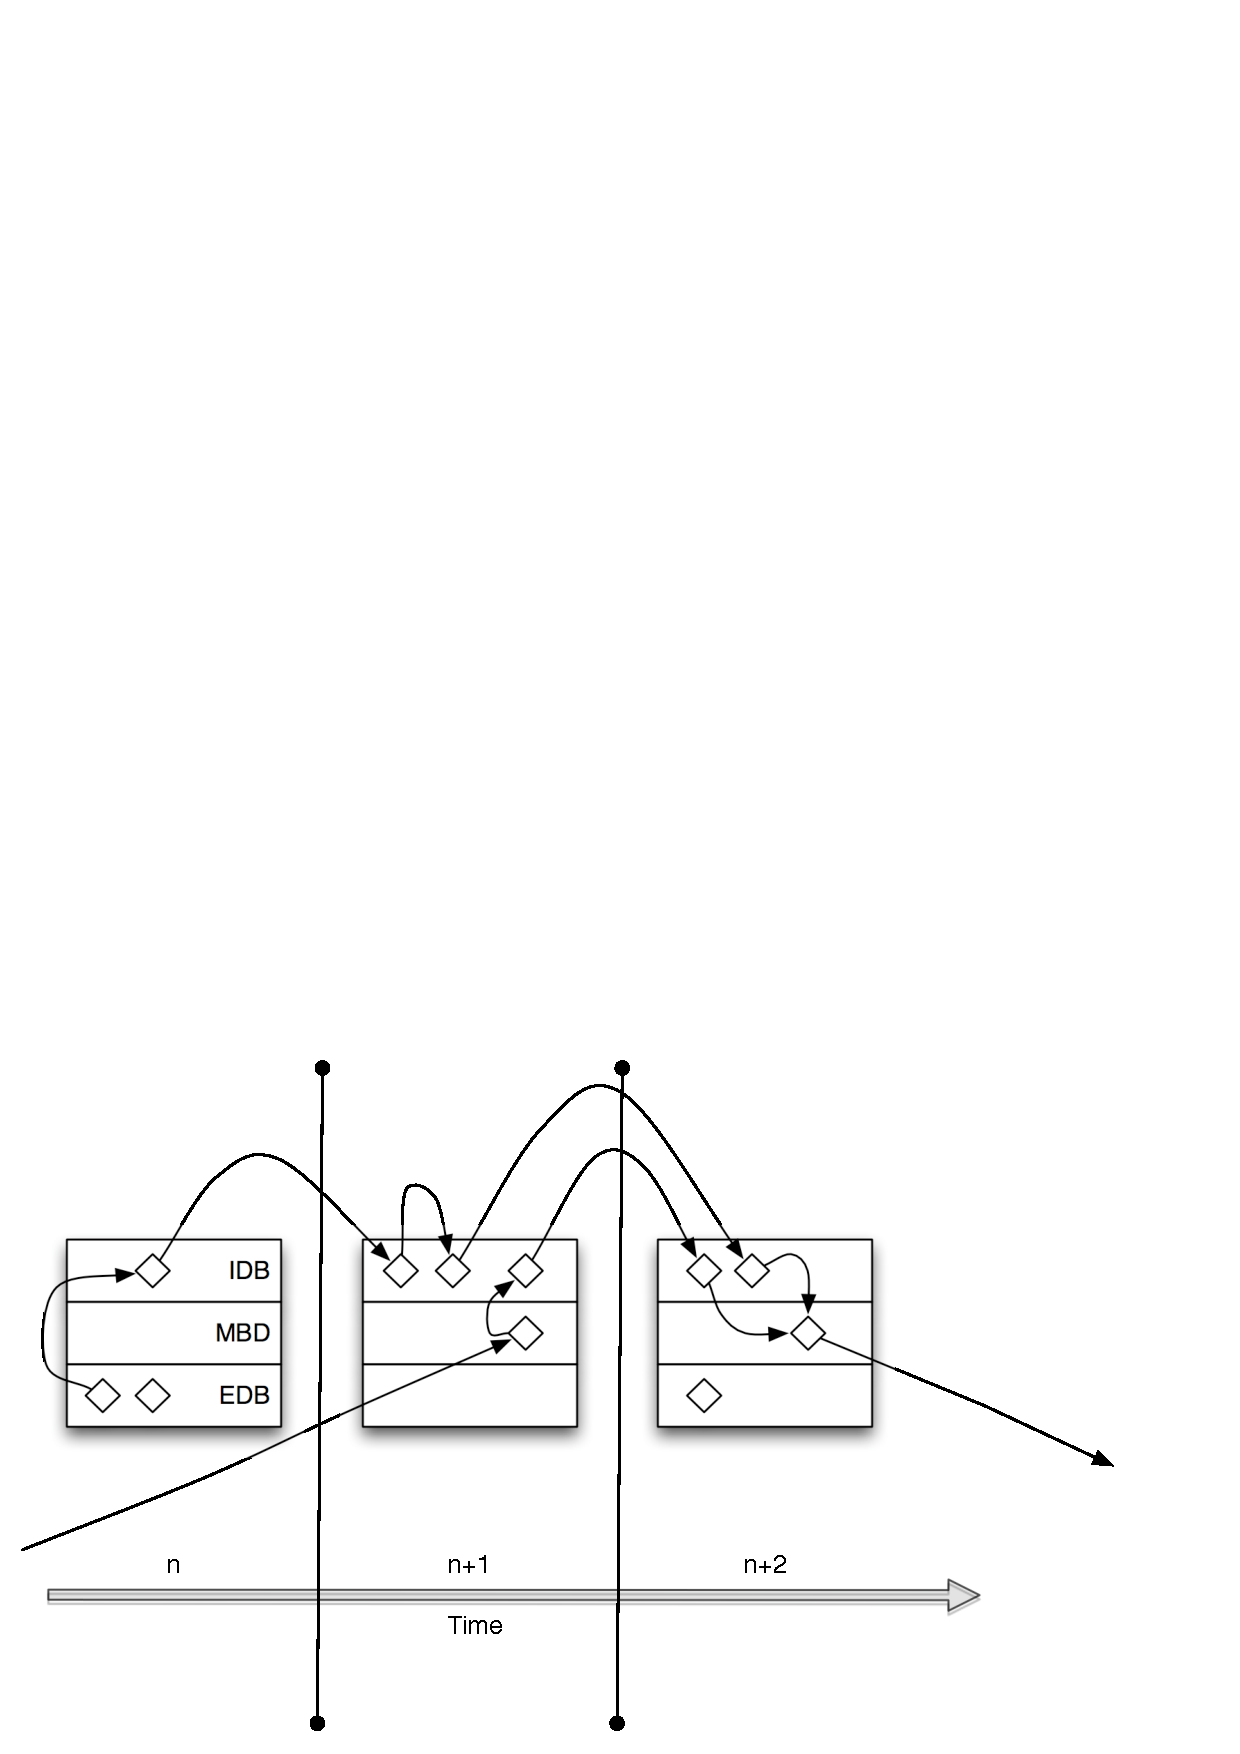
\includegraphics[width=1\linewidth]{figures/edbidbmdb.pdf}
  \label{fig:edbidbmdb}
  \caption{Derivations across time in IDB and MDB relations.}
\vspace{-8pt}
\end{figure}

\paa{this section (its placement \emph{and} content) is somewhat problematic given the current structure
of the draft.  We've established the notion of finite preambles of a (possibly infinite) EDB.  A trace is basically just
an interpretation (a set of ground atoms) -- by calling it a ``trace" we're connoting a post-hoc \wrm{warning: post hoc is undefined} interpretation.
A trace that is just EDB is sufficient, given a program, to augment the trace with IDB and MDB atoms such that
the resulting trace is a model (by simply running a fixpoint computation).  For a program with no async rules, the EDB of input is sufficient to recreate the
program execution exactly -- that is to say, to reproduce the single minimal model of the program given the EDB.
It is \emph{not} sufficient to recreate the execution of a program with async rules: intuitively, we'd need to include in 
the trace the complete MDB, for every entry in it potentially corresponds to one of many possible minimal models.
perhaps we just want to show that there is a method (drop the async rules and run a fixpoint computation to generate
the IDB from MDB and EDB) to regenerate a "complete trace" (ie minimal model) from EDB $\cup$ MDB}

%Consider a non-empty EDB $E$, an empty MBD $M$ and IDB $I$ and a program $P$.  Evaluating $P$ against $E$ may derive facts in $M$ and $I$.

\begin{definition}
A \emph{trace} is any set of facts from the EDB, NDB or IDB of a \lang program evaluation.
\end{definition}

Any trace for a \lang instance $(P,E)$ is an interpretation of $(P,E)$.
%\wrm{lol, why do we need the notion of an incomplete trace?}

\begin{definition}
%
A \emph{complete trace} of an evaluation of a \lang instance is the union of
the given EDB with the derived IDB and MDB.
%
\end{definition}

\begin{lemma}
%
A complete trace of a \lang instance $(P,E)$ is its unique minimal model.
%
\end{lemma}

%\begin{lemma}
%%
%For any bound on $successor$, a complete trace of a \lang  instance $(P,E)$ has a unique minimal model.
%%
%\end{lemma}

If we evaluate E given P, and P is stratifiable, the resulting set of ground atoms is a minimal model.
In our case, however, successor causes our EDB to be infinite, so the minimal model of any \lang program 
with temporal rules is potentially infinite.  \paa{but we'd like to show that a weaker property holds: that for any value $N$
in the \emph{successor} relation, the resulting program has a minimal model.}
\wrm{we either already showed this, or our theorems above are wrong.}


\begin{definition}
A \emph{minimal trace} is a subset of a complete trace that excludes any IDB ground atoms derived through an inductive
rule.
\end{definition}

A minimal trace of a \lang program $P$ is equivalent to the complete trace of which is is a subset -- the latter may be derived from the former by repeated
applications of inductive rules.  However, a given a \lang instance $(P, E)$ and a minimal trace T (where $E \subset T$), a fixpoint
computation will most likely \emph{not} yield a minimal model, because new tuples may be added to the MDB that represent a component 
of a different minimal model, and because these may affect the IDB.  The set of ground atoms $EDB \cup MDB_{old} \cup IDB_{new}$
\emph{may} may be a minimal model, iff $IDB_{new} = IDB_{old}$.  \paa{actually I am not sure if that is true}.  
$(EDB \cup MDB_{old} \cup IDB_{new} \cup IDB_{old})$ is certain to be a model, but is only minimal if $IDB_{new} \subset IDB_{old}$.

A minimal trace records the nondeterminism caused by the delay or reordering of async rules, and
is equivalent to the original program execution.  

\begin{definition}
A \emph{reduced trace} is a minimal trace with normalized time suffixes starting with 0 and increasing by 1 at each step.
\end{definition}

show a (trivial) procedure for reduction and make some claims about equivalences without entanglement.

\begin{definition}
A \emph{event trace} is a \lang EDB.
\end{definition}

An event trace and program P may be used to generate a new IDB and MDB.  The MDB is virtually certain to differ from that of another
execution, while the IDB may differ, depending on its dependency on the MDB.  The union of these three databases is of course a
minimal model, but probably not the same minimal model from another execution.  \paa{but can we say that it will often be true that if we project 
out the time attribute from every predicate, the minimal models will be the same? it won't always be true...}



\subsection{EDB Preambles}

\rcs{I've never seen someone use ``preamble'' to refer to this concept.  Why not call it a prefix?}

A \slang instance's EDB may be arbitrarily large.  In this section we introduce
the notion of a {\em preamble} -- a truncation of the EDB, and prove an
equivalence between full evaluation of a preamble and incremental evaluation
based on evaluation of an earlier preamble.
%A \slang instance may receive arbitrarily many external input tuples over the
%course of its execution, but should not wait arbitrarily long before
%performing deductions.  In this section we introduce the notion of EDB
%preambles, and prove an equivalence between two types of evaluation.

%In general, the EDB of a \slang instance may be infinite, and may lead to unsafe evaluations even when \emph{successor} is derived from it
%as in a post-hoc evaluation.

\begin{definition}
A \emph{preamble} $\alpha_{n}$ of an EDB $\Gamma$ is the set of facts in $\Gamma$ whose timestamp is less than or equal to $n$.
\end{definition}

If the EDB is finite, then it has a maximum timestamp $\top$, \rcs{is successor now part of the EDB? Otherwise, there is no max timestamp} and
$\alpha_{\top}$ = $\Gamma$.  \wrm{I don't think we use $\top$ anywhere else}
Because each preamble is a superset of all preambles with lower indices, we
have the monotonicity property:

$\forall \alpha_{i}, \alpha_{j} \in \Gamma : (i < j) \to (\alpha_{i} \subseteq \alpha_{j})$

%\paa{to your point, bill, I switched the lemma and proof below to one of IDB equivalence in the posthoc vs. continual interpretation
%rather than an inductive proof that every model in the series is minimal.  there is probably a very similar proof of the latter
%that we could include in the next section after introducing minimal models, stratification etc}

\wrm{todo: disuss replacing FP with some derivation tree thing}
\begin{definition}
%
Let $F$ be the set of all finite subsets of possible atoms.  Let $P$ be the set
of all finite subsets of possible rules.  Let $FP : P \times F \mapsto F$ be
the function representing the \emph{fixpoint} computation carried out by a
datalog interpreter.  That is, $FP_p$ takes an EDB to its corresponding IDB.
%
\end{definition}


\begin{lemma}
\label{lem:costmodel}
%
Let $i \in \mathbb{Z}$.  Then, $FP_p(\alpha_{i+1} \cup FP_p(\alpha_i)) =
FP_p(\alpha_{i+1})$.
%
\end{lemma}

%%this could (with some work) lead to an inductive proof
%%that an infinite model is minimal.  we could prove the (weaker?) property that
%%the infinite series of models of increasing finite preambles of an EDB are all 
%%minimal if one of them is.

\begin{proof}

%%Inductive step:

%%if we assume that some program P and finite preamble $\alpha_n$ of a trace $\Gamma$ produce a minimal model, 
%%then it follows that a preamble $\alpha_{n+1}$ and the IDB produced by the previous model produce a minimal model.

by contradiction. Assume $\exists i \in \mathbb{Z}$ such that:
$FP_p(\alpha_{i+1} \cup FP_p(\alpha_i)) \neq FP_p(\alpha_{i+1})$

{\bf Case 1:} $\exists A \in FP_p(\alpha_{i+1} \cup FP_p(\alpha_i)) : A \not\in FP_p(\alpha_{i+1}).$

This implies that $A$ is transitively dependent on atoms in $\alpha_{i+1} \cup
FP_p(\alpha_i)$.  However, if $A$ is transitively dependent only on atoms in
$\alpha_{i+1}$, then $A$ would be in $FP_p(\alpha_{i+1})$.  Thus, $A$ must be
transitively dependent on some atoms in $FP_p(\alpha_{i})$.  But $\alpha_{i}
\subset \alpha_{i+1}$, so this implies that $A$ is transitively dependent on
some atom in $\alpha_{i+1}$, which means $A \in FP_p(\alpha_{i+1})$.  This
contradicts our assumption, thus no such $A$ may exist.

{\bf Case 2:} $\exists A \in FP_p(\alpha_{i+1}) : A \not\in FP_p(\alpha_{i+1} \cup FP_p(\alpha_i)).$

This implies that $A$ is transitively dependent on $\alpha_{i+1}$.  In order
for $A \not\in FP_p(\alpha_{i+1} \cup FP_p(\alpha_i))$, we need $A$ to depend
negatively on an atom $B \in FP_p(\alpha_i)$.  But $B$ transitively depends on
an atom $C \in \alpha_i$.  $C \in \alpha_{i+1}$ by definition (if $B$ is
extensional, then $C=B$), so $B \in FP_p(\alpha_{i+1})$, so $a \not\in
FP_p(\alpha_{i+1})$.  This contradicts our assumption, thus no such $A$ may
exist.
%If $I_2 \neq I_3$, it must be the case that either there exists a ground atom in $I_2$ that is not in $I_3$, or that is in
%$I_3$ and not in $I_2$.  
%Take the former case first.  This means there is an atom $A$ that is entailed by P given $FP(\alpha_{j} \cup FP(\alpha_{i}))$
%but not entailed by P given $\alpha_{j}$, so it must be in $I_1$.   The only circumstances under which an atom in
%$I_1$ would not occur in the IDB $FP(\alpha_{j})$ is if there is a fact $B$ in $\alpha_{j}$ 
%corresponding to a negated subgoal in a rule $r$ in P upon which $A$ depends.  However, for this to occur, because a ground atom 
%in $I_1$ cannot depend upon a ground atom from the ``future", that fact $B$ would need to have occurred at some time less than 
%or equal to the to timestamp of atom $A$.  But this is not possible, because all timestamps in $\alpha_{j}$ that are not in any $\alpha_{k} | k<j$
%are strictly higher than any timestamps in $\alpha_{k}$.  Hence the first case leads to contradiction.
%As for the second case...
\end{proof}

\subsection{Cost Model}
%%\newdef{definition}{Definition}
Lemma~\ref{lem:costmodel} implies that we can trade computation cost for
storage cost in evaluation of a \slang program. 

%In the continuous interpretation of a \slang program, it is in general only
%useful to remember facts at a single timestamp in a predicate.  Two ways to
%approach this issue are to either always persist the ``latest'' version, or
%continuously re-derive the latest version.  These are represented in the naive
%deductive and overwriteable storage implementations below.

%\begin{figure}[t]
%\begin{tabular}{ll} \hline
%%Rule Pattern & Idiom & Prepare & Propose & Election \\ \hline \hline
%$d$ & Cost of a deductive step \\
%$s$ & Cost of storing a tuple \\
%$r$ & Cost of reading a tuple \\ 
%$t$ & Number of tuple derivations from deductive rules \\ 
%\hline
%$S$ & Set of tuples inserted \\
%$U$ & Set of tuples updated \\
%$P$ & Set of stored tuples, with time projected out \\ 
%$T$ & Set of stored tuple timestamps \\ 
%$Q$ & Set of query timestamps \\ \hline 
%\end{tabular}
%\caption{Cost model.}
%\label{fig:breakdown}
%\end{figure}


%\subsubsection{Naive Deductive Implementation}

%To evaluate a trace consisting of $S$ inserts and $U$ updates, a naive
%deductive implementation would:

%\begin{enumerate}
%
%\item
%
%\item
{\bf Naive Deductive Implementation: } We must evaluate every rule at time $1$
through $M$.  This implies persistent storage cost of $|\alpha_M|$, e.g. the
entire preamble up through $M$.
%A bottom-up evaluation of a predicate $P$ consists of evaluating all rules
%that reference $P$ in the head, and may involve polynomially many derivations
%in the size of the EDB up to time $M$.
A naive query plan for execution of a rule $R$ would take the cross product of
all body relations, $CP_R$, select the subset that matches the body conditions,
and project this subset onto the head predicate.  Assume each rule $R$ has an
associated selectivity from the cross product $s_R$, cost per each tuple in the
cross product $d_R$, and cost per each tuple in the subset selected from the
cross product $p_R$.  Each recursion is executed for a certain number of steps
steps.  This step has temporary storage and execution cost of:
%
\[ \sum_{t=0}^M \sum_{R} |CP_{(R,t)}|(p_{(R,t)} \cdot s_{(R,t)} + \cdot
d_{(R,t)}) \]
%
%\end{enumerate}

%In summary, the total execution cost is:

%\[ (S+2U)w + M \cdot \sum_{r : P \in r.head} n_r \cdot s_r \cdot d_r  \]

%Since we only need persist the EDB, the total storage cost is equal to the size
%of the EDB.

%$(|S|+2|U|)s + (|S|+2|U|)r + t + (\displaystyle\sum_{i=0}^{|Q|-1} \displaystyle\sum_{j=0}^{|T|-1} Q_{i} - T_{j})d$

%\subsubsection{Naive Overwriteable Storage Implementation}

%To evaluate a trace consisting of $S$ inserts and $U$ updates, a naive
%deductive implementation would:

%\begin{enumerate}
%
%\item
%Add all $I$ inserts, $D$ deletions, and $U$ updates to a log.  Note that
%an update consists of both an insertion and a deletion.  Assuming that
%inserting a fact into the EDB has some cost $w$ independent of the
%characteristics of the predicate (e.g. all predicates store their facts in hash
%tables), then this step has temporary storage and computation cost $(I+D+2U)w$.

{\bf Naive Overwriteable Storage Implementation: }An overwritable storage
implementation may trade some storage for better execution latency by storing
the most recent version of all predicates.  This implies persistent storage
cost of:
%
\[ |FP(\alpha_{M-1})| + |\alpha_M \cap \alpha_{M-1}| \]

We would need to evaluate every rule $R$ at timestamp $M$.  This entails
temporary storage and execution cost of:
%
\[ \sum_{R} |CP_{(R,M)}|(p_{(R,M)} \cdot s_{(R,M)} + d_{(R,M)}) \]
%This is in contrast to the
%naive deductive model, which would require computation from timestamp 1, but
%would not require persisting the IDB of the most recently computed stratum for
%each predicate.

%In summary, the total execution cost is:

%\[ (S+2U)w + \sum_{r} (M - Q_{r.head}) n_r \cdot s_r \cdot d_r  \]

%The total storage cost is the IDB of each predicate at its most recent
%timestamp.

%%\subsubsection{perhaps we can admit queries over the past that are bounded and pre-stated, and do GC}




\end{document}
